
\ifx\wholebook\relax \else
% ------------------------

\documentclass{article}
%------------------- Other types of document example ------------------------
%
%\documentclass[twocolumn]{IEEEtran-new}
%\documentclass[12pt,twoside,draft]{IEEEtran}
%\documentstyle[9pt,twocolumn,technote,twoside]{IEEEtran}
%
%-----------------------------------------------------------------------------
%%
% loading packages
%
\newif\ifpdf
\ifx\pdfoutput\undefined % We're not running pdftex
  \pdffalse
\else
  \pdftrue
\fi
%
%
\ifpdf
  \RequirePackage[pdftex,%
            CJKbookmarks,%
       bookmarksnumbered,%
              colorlinks,%
          linkcolor=blue,%
              hyperindex,%
        plainpages=false,%
       pdfstartview=FitH]{hyperref}
\else
  \RequirePackage[dvipdfm,%
             CJKbookmarks,%
        bookmarksnumbered,%
               colorlinks,%
           linkcolor=blue,%
               hyperindex,%
         plainpages=false,%
        pdfstartview=FitH]{hyperref}
  \AtBeginDvi{\special{pdf:tounicode GBK-EUC-UCS2}} % GBK -> Unicode
\fi
\usepackage{hyperref}

% other packages
%-----------------------------------------------------------------------------
\usepackage{graphicx, color}
\usepackage{CJK}
%
% for programming 
%
\usepackage{verbatim}
\usepackage{listings}


\lstdefinelanguage{Smalltalk}{
  morekeywords={self,super,true,false,nil,thisContext}, % This is overkill
  morestring=[d]',
  morecomment=[s]{"}{"},
  alsoletter={\#:},
  escapechar={!},
  literate=
    {BANG}{!}1
    {UNDERSCORE}{\_}1
    {\\st}{Smalltalk}9 % convenience -- in case \st occurs in code
    % {'}{{\textquotesingle}}1 % replaced by upquote=true in \lstset
    {_}{{$\leftarrow$}}1
    {>>>}{{\sep}}1
    {^}{{$\uparrow$}}1
    {~}{{$\sim$}}1
    {-}{{\sf -\hspace{-0.13em}-}}1  % the goal is to make - the same width as +
    %{+}{\raisebox{0.08ex}{+}}1		% and to raise + off the baseline to match -
    {-->}{{\quad$\longrightarrow$\quad}}3
	, % Don't forget the comma at the end!
  tabsize=2
}[keywords,comments,strings]

\lstloadlanguages{C++, Lisp, Smalltalk}

% ======================================================================

\def\BibTeX{{\rm B\kern-.05em{\sc i\kern-.025em b}\kern-.08em
    T\kern-.1667em\lower.7ex\hbox{E}\kern-.125emX}}

\newtheorem{theorem}{Theorem}

%
% mathematics
%
\newcommand{\be}{\begin{equation}}
\newcommand{\ee}{\end{equation}}
\newcommand{\bmat}[1]{\left( \begin{array}{#1} }
\newcommand{\emat}{\end{array} \right) }
\newcommand{\VEC}[1]{\mbox{\boldmath $#1$}}

% numbered equation array
\newcommand{\bea}{\begin{eqnarray}}
\newcommand{\eea}{\end{eqnarray}}

% equation array not numbered
\newcommand{\bean}{\begin{eqnarray*}}
\newcommand{\eean}{\end{eqnarray*}}

\RequirePackage{CJK,CJKnumb,CJKulem,CJKpunct}
% we use CJK as default environment
\AtBeginDocument{\begin{CJK*}{GBK}{song}\CJKtilde\CJKindent\CJKcaption{GB}}
\AtEndDocument{\clearpage\end{CJK*}}

%
% loading packages
%
\newif\ifpdf
\ifx\pdfoutput\undefined % We're not running pdftex
  \pdffalse
\else
  \pdftrue
\fi
%
%
\ifpdf
  \RequirePackage[pdftex,%
       bookmarksnumbered,%
              colorlinks,%
          linkcolor=blue,%
              hyperindex,%
        plainpages=false,%
       pdfstartview=FitH]{hyperref}
\else
  \RequirePackage[dvipdfm,%
        bookmarksnumbered,%
               colorlinks,%
           linkcolor=blue,%
               hyperindex,%
         plainpages=false,%
        pdfstartview=FitH]{hyperref}
\fi
\usepackage{hyperref}

% other packages
%-----------------------------------------------------------------------------
\usepackage{graphicx, color}
%
% for programming 
%
\usepackage{verbatim}
\usepackage{listings}
\usepackage{algorithmic} %for pseudocode
\usepackage{algorithm}


\lstdefinelanguage{Smalltalk}{
  morekeywords={self,super,true,false,nil,thisContext}, % This is overkill
  morestring=[d]',
  morecomment=[s]{"}{"},
  alsoletter={\#:},
  escapechar={!},
  literate=
    {BANG}{!}1
    {UNDERSCORE}{\_}1
    {\\st}{Smalltalk}9 % convenience -- in case \st occurs in code
    % {'}{{\textquotesingle}}1 % replaced by upquote=true in \lstset
    {_}{{$\leftarrow$}}1
    {>>>}{{\sep}}1
    {^}{{$\uparrow$}}1
    {~}{{$\sim$}}1
    {-}{{\sf -\hspace{-0.13em}-}}1  % the goal is to make - the same width as +
    %{+}{\raisebox{0.08ex}{+}}1		% and to raise + off the baseline to match -
    {-->}{{\quad$\longrightarrow$\quad}}3
	, % Don't forget the comma at the end!
  tabsize=2
}[keywords,comments,strings]

\lstloadlanguages{C++, Lisp, Haskell, Python, Smalltalk}

% ======================================================================

\def\BibTeX{{\rm B\kern-.05em{\sc i\kern-.025em b}\kern-.08em
    T\kern-.1667em\lower.7ex\hbox{E}\kern-.125emX}}

\newtheorem{theorem}{Theorem}

%
% mathematics
%
\newcommand{\be}{\begin{equation}}
\newcommand{\ee}{\end{equation}}
\newcommand{\bmat}[1]{\left( \begin{array}{#1} }
\newcommand{\emat}{\end{array} \right) }
\newcommand{\VEC}[1]{\mbox{\boldmath $#1$}}

% numbered equation array
\newcommand{\bea}{\begin{eqnarray}}
\newcommand{\eea}{\end{eqnarray}}

% equation array not numbered
\newcommand{\bean}{\begin{eqnarray*}}
\newcommand{\eean}{\end{eqnarray*}}




\setcounter{page}{1}

\begin{document}

%--------------------------

% ================================================================
%                 COVER PAGE
% ================================================================

\title{Binomial heap, Fibonacci heap, and pairing heap}

\author{Larry~LIU~Xinyu
\thanks{{\bfseries Larry LIU Xinyu } \newline
  Email: liuxinyu95@gmail.com \newline}
  }

\maketitle
\fi

\markboth{Binomial heap, Fibonacci heap, and pairing heap}{Elementary Algorithms}

\ifx\wholebook\relax
\chapter{Binomial heap, Fibonacci heap, and pairing heap}
\numberwithin{Exercise}{chapter}
\fi

% ================================================================
%                 Introduction
% ================================================================
\section{Introduction}
\label{introduction}
In previous chapter, we mentioned that heaps can be
generalized and implemented with varies of data structures. However,
only binary heaps are focused so far no matter by explicit binary
trees or implicit array.

It's quite natural to extend the binary tree to K-ary \cite{K-ary-tree} tree.
In this chapter, we first show Binomial heaps
which is actually consist of forest of K-ary trees. Binomial heaps gain the
performance for all operations to $O(\lg n)$, as well as keeping the finding
minimum element to $O(1)$ time.

If we delay some operations in Binomial
heaps by using lazy strategy, it turns to be Fibonacci heap.

All binary heaps we have shown perform
no less than $O(\lg n)$ time for merging, we'll show it's possible to
improve it to $O(1)$ with Fibonacci heap, which is quite helpful to
graph algorithms. Actually, Fibonacci heap achieves almost all operations
to good amortized time bound as $O(1)$,
and left the heap pop to $O(\lg n)$.

Finally, we'll introduce about the pairing heaps. It has the best performance in practice although the proof of it is still a conjecture for the time
being.


% ================================================================
%                 Binomial heap
% ================================================================
\section{Binomial Heaps}
\label{binomail-heap} \index{Binomial heap}


% ================================================================
%                 Definition
% ================================================================
\subsection{Definition}

Binomial heap is more complex than most of the binary heaps. However,
it has excellent merge performance which bound to $O(\lg n)$ time. A
binomial heap is consist of a list of binomial trees.

\subsubsection{Binomial tree}
\label{Binomial tree} \index{Binomial tree}

In order to explain why the name of the tree is `binomial', let's review
the famous Pascal's triangle (Also know as the Jia Xian's triangle to
memorize the Chinese methematican Jia Xian (1010-1070).)
\cite{wiki-pascal-triangle}.

\begin{verbatim}
    1
   1 1
  1 2 1
 1 3 3 1
1 4 6 4 1
...
\end{verbatim}

In each row, the numbers are all binomial coefficients. There are many
ways to gain a series of binomial coefficient numbers. One of them is
by using recursive composition. Binomial trees, as well, can be defined
in this way as the following.

\begin{itemize}
\item A binomial tree of rank 0 has only a node as the root;
\item A binomial tree of rank $n$ is consist of two rank $n-1$ binomial trees,
Among these 2 sub trees, the one has the bigger root element is linked as the
leftmost child of the other.
\end{itemize}

We denote a binomial tree of rank 0 as $B_0$, and the binomial tree of rank
$n$ as $B_n$.

Figure \ref{fig:link-bitree} shows a $B_0$ tree and how to link 2 $B_{n-1}$
trees to a $B_n$ tree.

\begin{figure}[htbp]
  \centering
  \subfloat[A $B_0$ tree.]{\hspace{0.1\textwidth}\includegraphics[scale=0.5]{img/b0tree.ps}\hspace{0.1\textwidth}} \\
  \subfloat[Linking 2 $B_{n-1}$ trees yields a $B_n$ tree.]{\includegraphics[scale=0.5]{img/link-bitree.ps}}
  \caption{Recursive definition of binomial trees} \label{fig:link-bitree}
\end{figure}

With this recursive definition, it easy to draw the form of binomial trees
of rank 0, 1, 2, ..., as shown in figure \ref{fig:bitree-forms}

\begin{figure}[htbp]
  \centering
  \subfloat[$B_0$ tree;]{\hspace{0.05\textwidth}\includegraphics[scale=0.5]{img/b0tree.ps}\hspace{0.05\textwidth}}
  \subfloat[$B_1$ tree;]{\hspace{0.05\textwidth}\includegraphics[scale=0.5]{img/b1tree.ps}\hspace{0.05\textwidth}}
  \subfloat[$B_2$ tree;]{\includegraphics[scale=0.5]{img/b2tree.ps}}
  \subfloat[$B_3$ tree;]{\includegraphics[scale=0.5]{img/b3tree.ps}} \\
  \subfloat[$B_4$ tree;]{\includegraphics[scale=0.5]{img/b4tree.ps}...}
  \caption{Forms of binomial trees with rank = 0, 1, 2, 3, 4, ...} \label{fig:bitree-forms}
\end{figure}

Observing the binomial trees reveals some interesting properties. For each rank $n$ binomial tree, if counting the number of nodes in each row, it can be found that it is the binomial number.

For instance for rank 4 binomial tree, there is 1 node as the root; and in the second level next to root, there are 4 nodes; and in 3rd level, there are 6 nodes; and in 4-th level, there are 4 nodes; and the 5-th level, there is 1 node. They are exactly 1, 4, 6, 4, 1 which is the 5th row in Pascal's triangle. That's why we call it binomial tree.

Another interesting property is that the total number of node for a binomial tree with rank $n$ is $2^n$. This can be proved either by binomial theory or the recursive definition directly.

\subsubsection{Binomial heap}
\label{Binomial heap} \index{Binomial heap!definition}

With binomial tree defined, we can introduce the definition of binomial heap. A binomial heap is a set of binomial trees (or a forest of binomial trees) that satisfied the following properties.

\begin{itemize}
\item Each binomial tree in the heap conforms to {\em heap property}, that the key of a node is equal or greater than the key of its parent. Here the heap is actually min-heap, for max-heap, it changes to `equal or less than'. In this chapter, we only discuss about min-heap, and max-heap can be equally applied by changing the comparison condition.
\item There is at most one binomial tree which has the rank $r$. In other words, there are no two binomial trees have the same rank.
\end{itemize}

This definition leads to an important result that for a binomial heap contains $n$ elements, and if convert $n$ to binary format yields $a_0, a_1, a_2, ..., a_m$, where $a_0$ is the LSB and $a_m$ is the MSB, then for each $0 \leq i \leq m$, if $a_i=0$, there is no binomial tree of rank $i$ and if $a_i = 1$, there must be a binomial tree of rank $i$.

For example, if a binomial heap contains 5 element, as 5 is `(LSB)101(MSB)', then there are 2 binomial trees in this heap, one tree has rank 0, the other has rank 2.

Figure \ref{fig:bheap2} shows a binomial heap which have 19 nodes, as 19 is `(LSB)11001(MSB)' in binary format, so there is a $B_0$ tree, a $B_1$ tree and a $B_4$ tree.

\begin{figure}[htbp]
  \centering
  \includegraphics[scale=0.5]{img/bheap2.ps}
  \caption{A binomial heap with 19 elements} \label{fig:bheap2}
\end{figure}

\subsubsection{Data layout}
\index{left child, right sibling}
There are two ways to define K-ary trees imperatively. One is by using
`left-child, right-sibling' approach\cite{CLRS}. It is compatible with
the typical binary tree structure. For each node, it has two fields,
left field and right field. We use the left field to point to the first
child of this node, and use the right field to point to the sibling
node of this node. All siblings are represented as a single directional
linked list. Figure \ref{fig:lcrs} shows an example tree represented in this way.

\begin{figure}[htbp]
  \centering
  \includegraphics[scale=0.5]{img/lcrs.ps}
  \caption{Example tree represented in `left-child, right-sibling' way. $R$ is the root node, it has no sibling, so it right side is pointed to $NIL$. $C_1, C_2, ..., C_n$ are children of $R$. $C_1$ is linked from the left side of $R$, other siblings of $C_1$ are linked one next to each other on the right side of $C_1$. $C_2', ..., C_m'$ are children of $C_1$.} \label{fig:lcrs}
\end{figure}

The other way is to use the library defined collection container, such
as array or list to represent all children of a node.

Since the rank of a tree plays very important role, we also defined
it as a field.

For `left-child, right-sibling' method, we defined the binomial tree
as the following.\footnote{C programs are also provided along with this book.}

\lstset{language=Python}
\begin{lstlisting}
class BinomialTree:
    def __init__(self, x = None):
        self.rank = 0
        self.key = x
        self.parent = None
        self.child = None
        self.sibling = None
\end{lstlisting}

When initialize a tree with a key, we create a leaf node, set its rank
as zero and all other fields are set as NIL.

It quite nature to utilize pre-defined list to represent multiple children
as below.

\begin{lstlisting}
class BinomialTree:
    def __init__(self, x = None):
        self.rank = 0
        self.key = x
        self.parent = None
        self.children = []
\end{lstlisting}

For purely functional settings, such as in Haskell language, binomial tree
are defined as the following.

\lstset{language=Haskell}
\begin{lstlisting}
data BiTree a = Node { rank :: Int
                     , root :: a
                     , children :: [BiTree a]}
\end{lstlisting}

While binomial heap are defined as a list of binomial trees (a forest) with
ranks in monotonically increase order. And as another implicit constraint,
there are no two binomial trees have the same rank.

\begin{lstlisting}
type BiHeap a = [BiTree a]
\end{lstlisting}

% ================================================================
%                 Basic heap operation
% ================================================================
\subsection{Basic heap operations}

\subsubsection{Linking trees}
\index{Binomial Heap!Linking}

Before dive into the basic heap operations such as pop and insert,
We'll first realize how to link two binomial trees with same rank into a
bigger one. According to the definition of binomial tree and heap
property that the root always contains the minimum key, we firstly
compare the two root values, select the smaller one as the new
root, and insert the other tree as the first child in front of
all other children. Suppose function $Key(T)$, $Children(T)$, and
$Rank(T)$ access the key, children and rank of a binomial tree
respectively.

\be
link(T_1, T_2) = \left \{
  \begin{array}
  {r@{\quad:\quad}l}
  node(r+1, x, \{ T_2 \} \cup C_1) & x < y \\
  node(r+1, y, \{ T_1 \} \cup C_2) & otherwise
  \end{array}
\right .
\label{eq:link}
\ee

Where

\[
  \begin{array}{l}
  x = Key(T_1) \\
  y = Key(T_2) \\
  r = Rank(T_1) = Rank(T_2) \\
  C_1 = Children(T_1) \\
  C_2 = Children(T_2)
  \end{array}
\]

\begin{figure}[htbp]
  \centering
  \includegraphics[scale=0.5]{img/link-bitree-xy.ps}
  \caption{Suppose $x < y$, insert $y$ as the first child of $x$.} \label{fig:link-xy}
\end{figure}

Note that the link operation is bound to $O(1)$ time if the $\cup$ is
a constant time operation. It's easy
to translate the link function to Haskell program as the following.

\lstset{language=Haskell}
\begin{lstlisting}
link :: (Ord a) => BiTree a -> BiTree a -> BiTree a
link t1@(Node r x c1) t2@(Node _ y c2) =
    if x<y then Node (r+1) x (t2:c1)
    else Node (r+1) y (t1:c2)
\end{lstlisting}

It's possible to realize the link operation in imperative way.
If we use `left child, right sibling' approach, we just link
the tree which has the bigger key to the left side of the other's
key, and link the children of it to the right side as sibling.
Figure \ref{fig:link-lcrs} shows the result of one case.

\begin{algorithmic}[1]
\Function{Link}{$T_1, T_2$}
  \If{\Call{Key}{$T_2$} $<$ \Call{Key}{$T_1$}}
    \State Exchange $T_1 \leftrightarrow T_2$
  \EndIf
  \State \Call{Sibling}{$T_2$} $\gets$ \Call{Child}{$T_1$}
  \State \Call{Child}{$T_1$} $\gets T_2$
  \State \Call{Parent}{$T_2$} $\gets T_1$
  \State \Call{Rank}{$T_1$} $\gets$ \Call{Rank}{$T_1$} + 1
  \State \Return $T_1$
\EndFunction
\end{algorithmic}

\begin{figure}[htbp]
  \centering
  \includegraphics[scale=0.5]{img/link-bitree-lcrs.ps}
  \caption{Suppose $x < y$, link $y$ to the left side of $x$ and link the original children of $x$ to the right side of $y$.} \label{fig:link-lcrs}
\end{figure}

And if we use a container to manage all children of a node, the
algorithm is like below.

\begin{algorithmic}[1]
\Function{Link'}{$T_1, T_2$}
  \If{\Call{Key}{$T_2$} $<$ \Call{Key}{$T_1$}}
    \State Exchange $T_1 \leftrightarrow T_2$
  \EndIf
  \State \Call{Parent}{$T_2$} $\gets T_1$
  \State \textproc{Insert-Before}(\Call{Children}{$T_1$}, $T_2$)
  \State \Call{Rank}{$T_1$} $\gets$ \Call{Rank}{$T_1$} + 1
  \State \Return $T_1$
\EndFunction
\end{algorithmic}

It's easy to translate both algorithms to real program. Here we only show the Python program of \textproc{Link'} for illustration purpose \footnote{The C and C++ programs are also available along with this book}.

\lstset{language=Python}
\begin{lstlisting}
def link(t1, t2):
    if t2.key < t1.key:
        (t1, t2) = (t2, t1)
    t2.parent = t1
    t1.children.insert(0, t2)
    t1.rank = t1.rank + 1
    return t1
\end{lstlisting}

\begin{Exercise}
Implement the tree-linking program in your favorite language with left-child, right-sibling method.
\end{Exercise}

\subsubsection*{}
We mentioned linking is a constant time algorithm and it is true
when using left-child,
right-sibling approach, However, if we use container to manage the
children, the performance depends on the concrete implementation of
the container. If it is plain array,
the linking time will be proportion to the number of children. In this
chapter, we assume the time is constant. This is true if the container
is implemented in linked-list.

\subsubsection{Insert a new element to the heap (push)}
\index{Binomial heap!insertion}
As the rank of binomial trees in a forest is monotonically increasing,
by using the $link$ function defined above, it's possible to define an
auxiliary function, so that we can insert a new tree, with rank no bigger
than the smallest one, to the heap which is a forest actually.

Denote the non-empty heap as $H = \{T_1, T_2, ..., T_n\}$, we define

\be
insertT(H, T) = \left \{
  \begin{array}
  {r@{\quad:\quad}l}
  \{ T \} & H = \phi \\
  \{ T \} \cup H & Rank(T) < Rank(T_1) \\
  insertT(H', link(T, T_1)) & otherwise
  \end{array}
\right .
\ee

where

\[
  H' = \{ T_2, T_3, ..., T_n\}
\]

The idea is that for the empty heap, we set the new tree as the only
element to create a singleton forest; otherwise, we compare the ranks
of the new tree and the first tree in the forest, if they are same,
we link them together, and recursively insert the linked result (a tree
with rank increased by one) to the rest of the forest; If they are
not same, since the pre-condition constraints the rank of the new
tree, it must be the smallest, we put this new tree in front of
all the other trees in the forest.

From the binomial properties mentioned above, there are at most
$O(\lg n)$ binomial trees in the forest, where $n$ is the total
number of nodes. Thus function $insertT$ performs at most $O(\lg n)$
times linking, which are all constant time operation. So the
performance of $insertT$ is $O(\lg n)$.
\footnote{There is interesting observation by comparing this
operation with adding two binary numbers. Which will lead to
topic of {\em numeric representation}\cite{okasaki-book}.}

The relative Haskell program is given as below.

\lstset{language=Haskell}
\begin{lstlisting}
insertTree :: (Ord a) => BiHeap a -> BiTree a -> BiHeap a
insertTree [] t = [t]
insertTree ts@(t':ts') t = if rank t < rank t' then t:ts
                           else insertTree ts' (link t t')
\end{lstlisting}

With this auxiliary function, it's easy to realize the insertion.
We can wrap the new element to be inserted as the only leaf of a tree,
then insert this tree to the binomial heap.

\be
insert(H, x) = insertT(H, node(0, x, \phi))
\ee

And we can continuously build a heap from a series of elements by folding.
For example the following Haskell define a helper function 'fromList'.

\begin{lstlisting}
fromList = foldl insert []
\end{lstlisting}

Since wrapping an element as a singleton tree takes $O(1)$ time,
the real work is done in $insertT$, the performance of binomial
heap insertion is bound to $O(\lg n)$.

The insertion algorithm can also be realized with imperative approach.

\begin{algorithm}
\caption{Insert a tree with 'left-child-right-sibling' method.}
\label{alg:insert-tree}
\begin{algorithmic}[1]
\Function{Insert-Tree}{$H, T$}
  \While{$H \neq \phi \land $ \textproc{Rank}(\Call{Head}{$H$}) = \Call{Rank}{$T$}}
    \State $(T_1, H) \gets$ \Call{Extract-Head}{$H$}
    \State $T \gets $ \Call{Link}{$T, T_1$}
  \EndWhile
  \State \Call{Sibling}{$T$} $\gets H$
  \State \Return $T$
\EndFunction
\end{algorithmic}
\end{algorithm}

Algorithm \ref{alg:insert-tree} continuously linking the first tree
in a heap with the new tree to be inserted if they have the same rank.
After that, it puts the linked-list of the rest trees as the sibling,
and returns the new linked-list.

If using a container to manage the children of a node, the algorithm
can be given in Algorithm \ref{alg:insert-tree1}.

\begin{algorithm}
\caption{Insert a tree with children managed by a container.}
\label{alg:insert-tree1}
\begin{algorithmic}[1]
\Function{Insert-Tree'}{$H, T$}
  \While{$H \neq \phi \land $ \Call{Rank}{$H[0]$} = \Call{Rank}{$T$}}
    \State $T_1 \gets$ \Call{Pop}{$H$}
    \State $T \gets $ \Call{Link}{$T, T_1$}
  \EndWhile
  \State \Call{Head-Insert}{$H, T$}
  \State \Return $H$
\EndFunction
\end{algorithmic}
\end{algorithm}

In this algorithm, function \textproc{Pop} removes the first tree
$T_1 = H[0]$ from the forest. And function \textproc{Head-Insert},
insert a new tree before any other trees in the heap, so that it
becomes the first element in the forest.

With either \textproc{Insert-Tree} or \textproc{Insert-Tree'} defined.
Realize the binomial heap insertion is trivial.

\begin{algorithm}
\caption{Imperative insert algorithm}
\label{alg:bheap-insert}
\begin{algorithmic}[1]
\Function{Insert}{$H, x$}
  \State \Return \textproc{Insert-Tree}($H$, \Call{Node}{$0, x, \phi$})
\EndFunction
\end{algorithmic}
\end{algorithm}

The following python program implement the insert algorithm by using
a container to manage sub-trees. the `left-child, right-sibling' program
is left as an exercise.

\lstset{language=Python}
\begin{lstlisting}
def insert_tree(ts, t):
    while ts !=[] and t.rank == ts[0].rank:
        t = link(t, ts.pop(0))
    ts.insert(0, t)
    return ts

def insert(h, x):
    return insert_tree(h, BinomialTree(x))
\end{lstlisting}

\begin{Exercise}
Write the insertion program in your favorite imperative programming
language by using the `left-child, right-sibling' approach.
\end{Exercise}

% =================================
%     Binomial heap merge
% =================================

\subsubsection{Merge two heaps}
\index{Binomial tree!merge}
When merge two binomial heaps, we actually try to merge two forests
of binomial trees. According to the definition, there can't be
two trees with the same rank and the ranks are in monotonically increasing
order. Our strategy is very similar to merge sort. That in every iteration,
we take the first tree from each forest, compare their ranks,
and pick the smaller one to the result heap; if the ranks are
equal, we then perform linking to get a new tree, and recursively
insert this new tree to the result of merging the rest trees.

Figure \ref{fig:merge-bheaps} illustrates the idea of this algorithm. This
method is different from the one given in \cite{CLRS}.

\begin{figure}[htbp]
  \centering
  \subfloat[Pick the tree with smaller rank to the result.]{\includegraphics[scale=0.7]{img/bheap-merge-1.ps}} \\
  \subfloat[If two trees have same rank, link them to a new tree, and recursively insert it to the merge result of the rest.]{\includegraphics[scale=0.7]{img/bheap-merge-2.ps}}
  \caption{Merge two heaps.} \label{fig:merge-bheaps}
\end{figure}

We can formalize this idea with a function. For non-empty cases, we
denote the two heaps as $H_1 = \{ T_1, T_2, ... \}$ and $H_2 = \{ T'_1, T'_2, ...\}$. Let $H'_1 = \{ T_2, T_3, ... \}$ and $H'_2 = \{ T'_2, T'_3, ... \}$.

\be
merge(H_1, H_2) = \left \{
  \begin{array}
  {r@{\quad:\quad}l}
  H_1 & H_2 = \phi \\
  H_2 & H_1 = \phi \\
  \{ T_1 \} \cup merge(H'_1, H_2) & Rank(T_1) < Rank(T'_1) \\
  \{ T'_1 \} \cup merge(H_1, H'_2) & Rank(T_1) > Rank(T'_1) \\
  insertT(merge(H'_1, H'_2), link(T_1, T'_1)) & otherwise
  \end{array}
\right .
\ee

To analysis the performance of merge, suppose there are $m_1$ trees in
$H_1$, and $m_2$ trees in $H_2$. There are at most $m_1 + m_2$ trees in
the merged result. If there are no two trees have the same rank, the
merge operation is bound to $O(m_1 + m_2)$. While if there need linking
for the trees with same rank, $insertT$ performs at most $O(m_1+m_2)$
time. Consider the fact that $m_1 = 1 + \lfloor \lg n_1 \rfloor$ and
$m_2 = 1 + \lfloor \lg n_2 \rfloor$, where
$n_1$, $n_2$ are the numbers of nodes in each heap, and
$\lfloor \lg n_1 \rfloor + \lfloor \lg n_2 \rfloor \leq 2 \lfloor \lg n \rfloor$, where $n = n_1 + n_2$, is the total number of nodes.
the final performance of merging is $O(\lg n)$.

Translating this algorithm to Haskell yields the following program.

\lstset{language=Haskell}
\begin{lstlisting}
merge:: (Ord a) => BiHeap a -> BiHeap a -> BiHeap a
merge ts1 [] = ts1
merge [] ts2 = ts2
merge ts1@(t1:ts1') ts2@(t2:ts2')
    | rank t1 < rank t2 = t1:(merge ts1' ts2)
    | rank t1 > rank t2 = t2:(merge ts1 ts2')
    | otherwise = insertTree (merge ts1' ts2') (link t1 t2)
\end{lstlisting}

Merge algorithm can also be described in imperative way as shown
in algorithm \ref{alg:bheap-merge}.

\begin{algorithm}
\caption{imperative merge two binomial heaps}
\label{alg:bheap-merge}
\begin{algorithmic}[1]
\Function{Merge}{$H_1, H_2$}
  \If{$H_1 = \phi$}
    \State \Return $H_2$
  \EndIf
  \If{$H_2 = \phi$}
    \State \Return $H_1$
  \EndIf
  \State $H \gets \phi$
  \While{$H_1 \neq \phi \land H_2 \neq \phi$}
    \State $T \gets \phi$
    \If{\Call{Rank}{$H_1$} $<$ \Call{Rank}{$H_2$}}
      \State $(T, H_1) \gets $ \Call{Extract-Head}{$H_1$}
    \ElsIf{\Call{Rank}{$H_2$} $<$ \Call{Rank}{$H_1$}}
      \State $(T, H_2) \gets $ \Call{Extract-Head}{$H_2$}
    \Else \Comment{Equal rank}
      \State $(T_1, H_1) \gets $ \Call{Extract-Head}{$H_1$}
      \State $(T_2, H_2) \gets $ \Call{Extract-Head}{$H_2$}
      \State $T \gets $ \Call{Link}{$T_1, T_2$}
    \EndIf
    \State \Call{Append-Tree}{$H, T$}
  \EndWhile
  \If{$H_1 \neq \phi$}
    \State \Call{Append-Trees}{$H, H_1$}
  \EndIf
  \If{$H_2 \neq \phi$}
    \State \Call{Append-Trees}{$H, H_2$}
  \EndIf
  \State \Return $H$
\EndFunction
\end{algorithmic}
\end{algorithm}

Since both heaps contain binomial trees with rank in monotonically
increasing order. Each iteration, we pick the tree with smallest
rank and append it to the result heap. If both trees have same rank
we perform linking first. Consider the \textproc{Append-Tree} algorithm,
The rank of the new tree to be appended, can't be less than
any other trees in the result heap according to our merge strategy,
however, it might be equal to the rank of the last tree in the
result heap. This can happen if the last tree appended are the
result of linking, which will increase the rank by one. In this
case, we must link the new tree to be inserted with the last tree.
In below algorithm, suppose function \textproc{Last}($H$) refers
to the last tree in a heap, and \textproc{Append}($H, T$) just
appends a new tree at the end of a forest.

\begin{algorithmic}[1]
\Function{Append-Tree}{$H, T$}
  \If{$H \neq \phi \land$ \Call{Rank}{$T$} $=$ \textproc{Rank}(\Call{Last}{$H$})}
    \State \Call{Last}{$H$} $\gets$ \textproc{Link}($T$, \Call{Last}{$H$})
  \Else
    \State \Call{Append}{$H, T$}
  \EndIf
\EndFunction
\end{algorithmic}

Function \textproc{Append-Trees} repeatedly call this function, so
that it can append all trees in a heap to the other heap.

\begin{algorithmic}[1]
\Function{Append-Trees}{$H_1, H_2$}
  \For{each $T \in H_2$}
    \State $H_1 \gets $ \Call{Append-Tree}{$H_1, T$}
  \EndFor
\EndFunction
\end{algorithmic}

The following Python program translates the merge algorithm.

\lstset{language=Python}
\begin{lstlisting}
def append_tree(ts, t):
    if ts != [] and ts[-1].rank == t.rank:
        ts[-1] = link(ts[-1], t)
    else:
        ts.append(t)
    return ts

def append_trees(ts1, ts2):
    return reduce(append_tree, ts2, ts1)

def merge(ts1, ts2):
    if ts1 == []:
        return ts2
    if ts2 == []:
        return ts1
    ts = []
    while ts1 != [] and ts2 != []:
        t = None
        if ts1[0].rank < ts2[0].rank:
            t = ts1.pop(0)
        elif ts2[0].rank < ts1[0].rank:
            t = ts2.pop(0)
        else:
            t = link(ts1.pop(0), ts2.pop(0))
        ts = append_tree(ts, t)
    ts = append_trees(ts, ts1)
    ts = append_trees(ts, ts2)
    return ts
\end{lstlisting}

\begin{Exercise}

The program given above uses a container to manage sub-trees.
Implement the merge algorithm in your favorite imperative programming
language with `left-child, right-sibling' approach.

\end{Exercise}

\subsubsection{Pop}
\index{Binomial heap!pop}
Among the forest which forms the binomial heap, each binomial tree
conforms to heap property that the root contains the minimum element
in that tree. However, the order relationship of these roots can be
arbitrary. To find the minimum element in the heap, we can select the
smallest root of these trees. Since there are $\lg n$ binomial trees,
this approach takes $O(\lg n)$ time.

However, after we locate the minimum element (which is also know as
the top element of a heap), we need remove it from the heap and keep
the binomial property to accomplish heap-pop operation.
Suppose the forest forms the binomial heap consists trees of
$B_i, B_j, ..., B_p, ..., B_m$, where $B_k$ is a binomial tree of
rank $k$, and the minimum element is the root of $B_p$. If we
delete it, there will be $p$ children left, which are all
binomial trees with ranks $p-1, p-2, ..., 0$.

One tool at hand is that we have defined $O(\lg n)$ merge function.
A possible approach is to reverse the $p$ children, so that their
ranks change to monotonically increasing order, and forms a binomial
heap $H_p$. The rest of trees is still a binomial
heap, we represent it as $H' = H - B_p$. Merging $H_p$ and $H'$ given
the final result of pop. Figure \ref{fig:bheap-del-min} illustrates
this idea.

\begin{figure}[htbp]
  \centering
  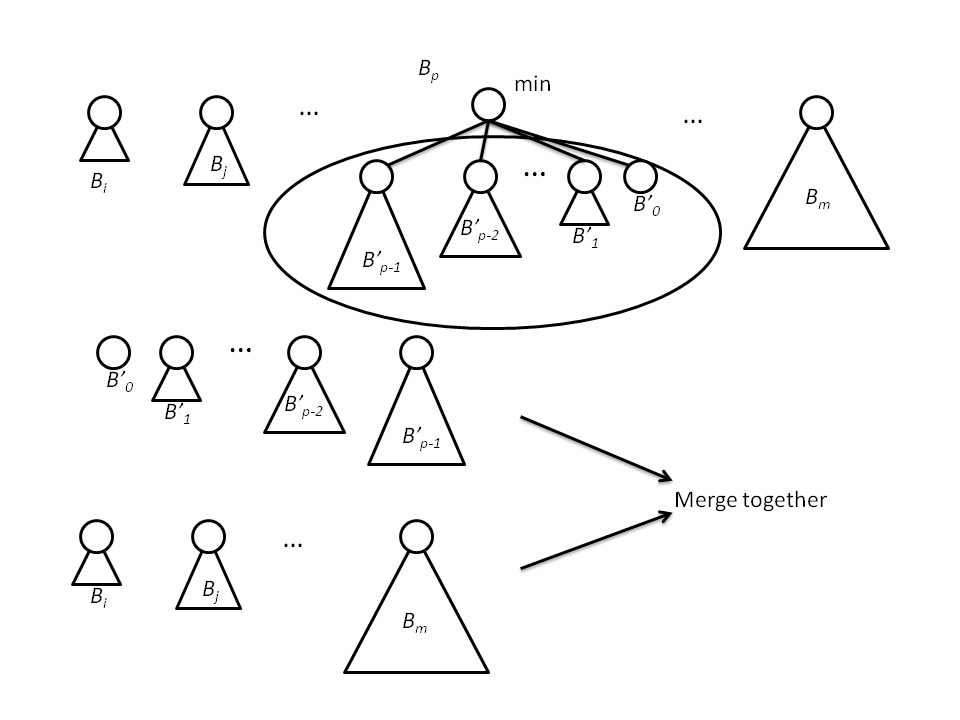
\includegraphics[scale=0.5]{img/bheap-pop.eps}
  \caption{Pop the minimum element from a binomial heap.}
  \label{fig:bheap-del-min}
\end{figure}

In order to realize this algorithm, we first need to define an
auxiliary function, which can extract the tree contains the minimum
element at root from the forest.

\be
extractMin(H) = \left \{
  \begin{array}
  {r@{\quad:\quad}l}
  (T, \phi) & \text{H is a singleton as } \{ T \} \\
  (T_1, H') & Root(T_1) < Root(T') \\
  (T', \{T_1\} \cup H'') & otherwise
  \end{array}
\right .
\ee

where

\[
  \begin{array}{lr}
  H = \{ T_1, T_2, ...\} & \text{for the non-empty forest case;} \\
  H' = \{ T_2, T_3, ...\} & \text{is the forest without the first tree;} \\
  (T', H'') = extractMin(H')
  \end{array}
\]

The result of this function is a tuple. The first part is the
tree which has the minimum element at root, the second part is
the rest of the trees after remove the first part from the forest.

This function examine each of the trees in the forest thus is bound
to $O(\lg n)$ time.

The relative Haskell program can be give respectively.

\lstset{language=Haskell}
\begin{lstlisting}
extractMin :: (Ord a) => BiHeap a -> (BiTree a, BiHeap a)
extractMin [t] = (t, [])
extractMin (t:ts) = if root t < root t' then (t, ts)
                    else (t', t:ts')
    where
      (t', ts') = extractMin ts
\end{lstlisting}

With this function defined, to return the minimum element is trivial.

\begin{lstlisting}
findMin :: (Ord a) => BiHeap a -> a
findMin = root . fst. extractMin
\end{lstlisting}

Of course, it's possible to just traverse forest and pick the
minimum root without remove the tree for this purpose. Below
imperative algorithm describes it with `left child, right sibling'
approach.

\begin{algorithmic}[1]
\Function{Find-Minimum}{$H$}
  \State $T \gets $ \Call{Head}{$H$}
  \State $min \gets \infty$
  \While{$T \ne \phi$}
    \If{\Call{Key}{$T$}$ < min$}
      \State $min \gets $ \Call{Key}{$T$}
    \EndIf
    \State $T \gets $ \Call{Sibling}{$T$}
  \EndWhile
  \State \Return $min$
\EndFunction
\end{algorithmic}

While if we manage the children with collection containers, the link
list traversing is abstracted as to find the minimum element among the list.
The following Python program shows about this situation.

\lstset{language=Python}
\begin{lstlisting}
def find_min(ts):
    min_t = min(ts, key=lambda t: t.key)
    return min_t.key
\end{lstlisting}

Next we define the function to delete the minimum element from
the heap by using $extractMin$.

\be
delteMin(H) = merge(reverse(Children(T)), H')
\ee

where

\[
  (T, H') = extractMin(H)
\]

Translate the formula to Haskell program is trivial and we'll skip
it.

To realize the algorithm in procedural way takes extra efforts
including list reversing etc. We left these details as exercise to the
reader. The following pseudo code illustrate the imperative
pop algorithm

\begin{algorithmic}[1]
\Function{Extract-Min}{$H$}
  \State $(T_{min}, H) \gets$ \Call{Extract-Min-Tree}{$H$}
  \State $H \gets$ \textproc{Merge}($H$, \textproc{Reverse}(\Call{Children}{$T_{min}$}))
  \State \Return (\Call{Key}{$T_{min}$}, $H$)
\EndFunction
\end{algorithmic}

With pop operation defined, we can realize heap sort by creating
a binomial heap from a series of numbers, than keep popping the
smallest number from the heap till it becomes empty.

\be
sort(xs) = heapSort(fromList(xs))
\ee

And the real work is done in function $heapSort$.

\be
heapSort(H) = \left \{
  \begin{array}
  {r@{\quad:\quad}l}
  \phi & H = \phi \\
  \{ findMin(H)  \} \cup heapSort(deleteMin(H)) & otherwise
  \end{array}
\right .
\ee

Translate to Haskell yields the following program.

\lstset{language=Haskell}
\begin{lstlisting}
heapSort :: (Ord a) => [a] -> [a]
heapSort = hsort . fromList where
    hsort [] = []
    hsort h = (findMin h):(hsort $ deleteMin h)
\end{lstlisting} %$

Function fromList can be defined by folding. Heap sort can
also be expressed in procedural way respectively. Please refer to
previous chapter about binary heap for detail.

\begin{Exercise}
\begin{itemize}
\item Write the program to return the minimum element from a
binomial heap in your favorite imperative programming language
with 'left-child, right-sibling' approach.

\item Realize the \textproc{Extract-Min-Tree}() Algorithm.

\item For 'left-child, right-sibling' approach, reversing all
children of a tree is actually reversing a single-direct linked-list.
Write a program to reverse such linked-list in your favorite
imperative programming language.
\end{itemize}
\end{Exercise}

\subsubsection{More words about binomial heap}
As what we have shown that insertion and merge are bound to $O(\lg n)$
time. The results are all ensure for the {\em worst case}. The
amortized performance are $O(1)$. We skip the proof for this
fact.

% ================================================================
%                 Fibonacci heaps
% ================================================================
\section{Fibonacci Heaps}
\label{fib-heap} \index{Fibonacci Heap}

It's interesting that why the name is given as `Fibonacci heap'.
In fact, there is no direct connection from the structure design
to Fibonacci series. The inventors of `Fibonacci heap', Michael L.
Fredman and Robert E. Tarjan, utilized the property of Fibonacci series
to prove the performance time bound, so they decided to use Fibonacci
to name this data structure.\cite{CLRS}

% ================================================================
%                 Definition
% ================================================================
\subsection{Definition}

Fibonacci heap is essentially a lazy evaluated binomial heap. Note
that, it doesn't mean implementing binomial heap in lazy evaluation
settings, for instance Haskell, brings Fibonacci heap automatically.
However, lazy evaluation setting does help in realization. For example
in \cite{hackage-fibq}, presents a elegant implementation.

Fibonacci heap has excellent performance theoretically. All operations
except for pop are bound to amortized $O(1)$ time. In this section,
we'll give an algorithm different from some popular textbook\cite{CLRS}.
Most of the ideas present here are based on Okasaki's work\cite{okasaki-fibh}.

Let's review and compare the performance of binomial heap and Fibonacci
heap (more precisely, the performance goal of Fibonacci heap).

% \begin{table}
% \caption{Performance goal of Fibonacci heap}
\begin{tabular}{l | c | r}
  \hline
  operation & Binomial heap & Fibonacci heap \\
  \hline
  insertion & $O(\lg n)$ & $O(1)$ \\
  merge & $O(\lg n)$ & $O(1)$ \\
  top & $O(\lg n)$ & $O(1)$ \\
  pop & $O(\lg n)$ & amortized $O(\lg n)$ \\
  \hline
\end{tabular}
% \end{table}

Consider where is the bottleneck of inserting a new element $x$ to
binomial heap. We actually wrap $x$ as a singleton leaf and insert
this tree into the heap which is actually a forest.

During this operation, we inserted the tree in
monotonically increasing order of rank, and once the rank is equal,
recursively linking and inserting will happen, which lead to the
$O(\lg n)$ time.

As the lazy strategy, we can postpone the ordered-rank insertion and
merging operations. On the contrary, we just put the singleton
leaf to the forest. The problem is that when we try to find the
minimum element, for example the top operation, the performance
will be bad, because we need check all trees in the forest, and
there aren't only $O(\lg n)$ trees.

In order to locate the top element in constant time, we must remember
where is the tree contains the minimum element as root.

Based on this idea, we can reuse the definition of binomial tree
and give the definition of Fibonacci heap as the following Haskell
program for example.

\lstset{language=Haskell}
\begin{lstlisting}
data BiTree a = Node { rank :: Int
                     , root :: a
                     , children :: [BiTree a]}
\end{lstlisting}

The Fibonacci heap is either empty or a forest of binomial trees with
the minimum element stored in a special one explicitly.

\begin{lstlisting}
data FibHeap a = E | FH { size :: Int
                        , minTree :: BiTree a
                        , trees :: [BiTree a]}
\end{lstlisting}

For convenient purpose, we also add a size field to record how many
elements are there in a heap.

The data layout can also be defined in imperative way as the following
ANSI C code.

\lstset{language=C}
\begin{lstlisting}
struct node{
  Key key;
  struct node *next, *prev, *parent, *children;
  int degree; /* As known as rank */
  int mark;
};

struct FibHeap{
  struct node *roots;
  struct node *minTr;
  int n; /* number of nodes */
};
\end{lstlisting}

For generality, Key can be a customized type, we use integer for illustration
purpose.

\lstset{language=C}
\begin{lstlisting}
typedef int Key;
\end{lstlisting}

In this chapter, we use the circular doubly linked-list for imperative
settings to realize the Fibonacci Heap as described in \cite{CLRS}.
It makes many operations easy and fast. Note that, there are two extra
fields added. A $degree$ also known as $rank$ for a node is the number
of children of this node; Flag $mark$ is used only in decreasing key
operation. It will be explained in detail in later section.


% ================================================================
%          Basic Heap operations
% ================================================================
\subsection{Basic heap operations}
As we mentioned that Fibonacci heap is essentially binomial heap
implemented in a lazy evaluation strategy, we'll reuse many algorithms
defined for binomial heap.

\subsubsection{Insert a new element to the heap}
\index{Fibonacci Heap!insert}
Recall the insertion algorithm of binomial  tree. It can be treated
as a special case of merge operation, that one heap contains only
a singleton tree. So that the inserting algorithm can be defined
by means of merging.

\be
insert(H, x) = merge(H, singleton(x))
\label{eq:fib-insert}
\ee

where singleton is an auxiliary function to wrap an element to a
one-leaf-tree.

\[
singleton(x) = FibHeap(1, node(1, x, \phi), \phi)
\]

Note that function $FibHeap()$ accepts three parameters, a
size value, which is 1 for this one-leaf-tree, a special tree
which contains the minimum element as root, and a list of other
binomial trees in the forest. The meaning of function $node()$ is
as same as before, that it creates a binomial tree from a rank,
an element, and a list of children.

Insertion can also be realized directly by appending the new node
to the forest and updated the record of the tree which contains the
minimum element.

\begin{algorithmic}[1]
\Function{Insert}{$H, k$}
  \State $x \gets$ \Call{Singleton}{$k$} \Comment{Wrap $x$ to a node}
  \State append $x$ to root list of $H$
  \If{$T_{min}(H) = NIL \lor k <$ \Call{Key}{$T_{min}(H)$} }
    \State $T_{min}(H) \gets x$
  \EndIf
  \State \Call{n}{$H$} $\gets$ \Call{n}{$H$}+1
\EndFunction
\end{algorithmic}

Where function $T_{min}()$ returns the tree which contains the minimum
element at root.

The following C source snippet is a translation for this algorithm.

\lstset{language=C}
\begin{lstlisting}
struct FibHeap* insert_node(struct FibHeap* h, struct node* x){
  h = add_tree(h, x);
  if(h->minTr == NULL || x->key < h->minTr->key)
    h->minTr = x;
  h->n++;
  return h;
}
\end{lstlisting}

\begin{Exercise}
Implement the insert algorithm in your favorite imperative programming
language completely. This is also an exercise to circular doubly linked list
manipulation.
\end{Exercise}

\subsubsection{Merge two heaps}
\index{Fibonacci Heap!merge}
Different with the merging algorithm of binomial heap, we post-pone
the linking operations later. The idea is to just put all binomial
trees from each heap together, and choose one special tree which
record the minimum element for the result heap.

\be
merge(H_1, H_2) = \left \{
  \begin{array}
  {r@{\quad:\quad}l}
  H_1 & H_2 = \phi \\
  H_2 & H_1 = \phi \\
  FibHeap(s_1 + s_2, {T_1}_{min}, \{ {T_2}_{min} \} \cup \mathbb{T}_1 \cup \mathbb{T}_2) & root({T_1}_{min}) < root({T_2}_{min}) \\
  FibHeap(s_1 + s_2, {T_2}_{min}, \{ {T_1}_{min} \} \cup \mathbb{T}_1 \cup \mathbb{T}_2) & otherwise \\
  \end{array}
\right .
\ee

where $s_1$ and $s_2$ are the size of $H_1$ and $H_2$; ${T_1}_{min}$ and
${T_2}_{min}$ are the special trees with minimum element as root in $H_1$
and $H_2$ respectively; $\mathbb{T}_1 = \{{T_1}_1, {T_1}_2, ...\}$ is
a forest contains all other binomial trees in $H_1$; while $\mathbb{T}_2$
has the same meaning as $\mathbb{T}_1$ except that it represents the
forest in $H_2$. Function $root(T)$ return the root element of a binomial
tree.

Note that as long as the $\cup$ operation takes constant time, these
$merge$ algorithm is bound to $O(1)$. The following Haskell program
is the translation of this algorithm.

\lstset{language=Haskell}
\begin{lstlisting}
merge:: (Ord a) => FibHeap a -> FibHeap a -> FibHeap a
merge h E = h
merge E h = h
merge h1@(FH sz1 minTr1 ts1) h2@(FH sz2 minTr2 ts2)
    | root minTr1 < root minTr2 = FH (sz1+sz2) minTr1 (minTr2:ts2++ts1)
    | otherwise = FH (sz1+sz2) minTr2 (minTr1:ts1++ts2)
\end{lstlisting}

Merge algorithm can also be realized imperatively by concatenating
the root lists of the two heaps.

\begin{algorithmic}[1]
\Function{Merge}{$H_1, H_2$}
  \State $H \gets \Phi$
  \State \Call{Root}{$H$} $\gets$ \textproc{Concat}(\Call{Root}{$H_1$}, \Call{Root}{$H_2$})
  \If{\Call{Key}{$T_{min}(H_1)$} $<$ \Call{Key}{$T_{min}(H_2)$}}
    \State $T_{min}(H) \gets T_{min}(H_1)$
  \Else
    \State $T_{min}(H) \gets T_{min}(H_2)$
  \EndIf
  \Call{n}{$H$} = \Call{n}{$H_1$} + \Call{n}{$H_2$}
  \State release $H_1$ and $H_2$
  \State \Return $H$
\EndFunction
\end{algorithmic}

This function assumes neither $H_1$, nor $H_2$ is empty. And it's easy
to add handling to these special cases as the following ANSI C program.

\lstset{language=C}
\begin{lstlisting}
struct FibHeap* merge(struct FibHeap* h1, struct FibHeap* h2){
  struct FibHeap* h;
  if(is_empty(h1))
    return h2;
  if(is_empty(h2))
    return h1;
  h = empty();
  h->roots = concat(h1->roots, h2->roots);
  if(h1->minTr->key < h2->minTr->key)
    h->minTr = h1->minTr;
  else
    h->minTr = h2->minTr;
  h->n = h1->n + h2->n;
  free(h1);
  free(h2);
  return h;
}
\end{lstlisting}

With $merge$ function defined, the $O(1)$ insertion algorithm is realized
as well. And we can also give the $O(1)$ time top function as below.

\be
top(H) = root(T_{min})
\ee

\begin{Exercise}
Implement the circular doubly linked list concatenation function in
your favorite imperative programming language.
\end{Exercise}

\subsubsection{Extract the minimum element from the heap (pop)}
\index{Fibonacci Heap!pop} \index{Fibonacci Heap!delete min}

The pop (delete the minimum element) operation is the most complex
one in Fibonacci heap. Since we postpone the tree consolidation
in merge algorithm. We have to compensate it somewhere. Pop is
the only place left as we have defined, insert, merge, top already.

There is an elegant procedural algorithm to do the tree consolidation
by using an auxiliary array\cite{CLRS}. We'll show it later in imperative
approach section.

In order to realize the purely functional consolidation algorithm,
let's first consider a similar number puzzle.

Given a list of numbers, such as $\{2, 1, 1, 4, 8, 1, 1, 2, 4\}$, we want
to add any two values if they are same. And repeat this procedure till
all numbers are unique. The result of the example list should be
$\{8, 16\}$ for instance.

One solution to this problem will as the following.

\be
consolidate(L) = fold(meld, \phi, L)
\ee

Where $fold()$ function is defined to iterate all elements from a list,
applying a specified function to the intermediate result and each
element. it is sometimes called as {\em reducing}. Please refer to the
chapter of binary search tree for it.

$L=\{x_1, x_2, ..., x_n\}$, denotes a list of numbers; and we'll use
$L'=\{x_2, x_3, ..., x_n\}$ to represent the rest of the list with the
first element removed. Function $meld()$ is defined as below.

\be
meld(L, x) = \left \{
  \begin{array}
  {r@{\quad:\quad}l}
  \{ x \} & L = \phi \\
  meld(L', x+x_1) & x = x_1 \\
  \{ x \} \cup L & x < x_1 \\
  \{ x_1 \} \cup meld(L', x) & otherwise
  \end{array}
\right .
\ee

The $consolidate()$ function works as the follows. It maintains an
ordered result list $L$, contains only unique numbers, which is
initialized from an empty list $\phi$. Each time it process an
element $x$, it firstly check if the first element in $L$ is equal
to $x$, if so, it will add them together (which yields $2x$),
and repeatedly check if $2x$ is equal to the next element in $L$.
This process won't stop until either the element to be melt is
not equal to the head element in the rest of the list, or the
list becomes empty. Table \ref{tb:num-consolidate} illustrates
the process of consolidating number sequence $\{2, 1, 1, 4, 8, 1, 1, 2, 4\}$.
Column one lists the number 'scanned' one by one; Column two
shows the intermediate result, typically the new scanned number
is compared with the first number in result list. If they
are equal, they are enclosed in a pair of parentheses; The
last column is the result of meld, and it will be used as the
input to next step processing.

The Haskell program can be give accordingly.

\lstset{language=Haskell}
\begin{lstlisting}
consolidate = foldl meld [] where
    meld [] x = [x]
    meld (x':xs) x | x == x' = meld xs (x+x')
                   | x < x'  = x:x':xs
                   | otherwise = x': meld xs x
\end{lstlisting}

We'll analyze the performance of consolidation as a part of
pop operation in later section.

\begin{table}
\caption{Steps of consolidate numbers} \label{tb:num-consolidate}
\centering
\begin{tabular}{r | l | l }
  \hline
  number & intermediate result & result \\
  \hline
  2 & 2 & 2 \\
  1 & 1, 2 & 1, 2 \\
  1 & (1+1), 2 & 4 \\
  4 & (4+4) & 8 \\
  8 & (8+8) & 16 \\
  1 & 1, 16 & 1, 16 \\
  1 & (1+1), 16 & 2, 16 \\
  2 & (2+2), 16 & 4, 16 \\
  4 & (4+4), 16 & 8, 16 \\
  \hline
\end{tabular}
\end{table}

The tree consolidation is very similar to this algorithm except
it performs based on rank. The only thing we need to do is to
modify $meld()$ function a bit, so that it compare on ranks and
do linking instead of adding.

\be
meld(L, x) = \left \{
  \begin{array}
  {r@{\quad:\quad}l}
  \{ x \} & L = \phi \\
  meld(L', link(x, x_1)) & rank(x) = rank(x_1) \\
  \{ x \} \cup L & rank(x) < rank(x_1) \\
  \{ x_1 \} \cup meld(L', x) & otherwise
  \end{array}
\right .
\ee

The final consolidate Haskell program changes to the below version.

\lstset{language=Haskell}
\begin{lstlisting}
consolidate :: (Ord a) => [BiTree a] -> [BiTree a]
consolidate = foldl meld [] where
    meld [] t = [t]
    meld (t':ts) t | rank t == rank t' = meld ts (link t t')
                   | rank t <  rank t' = t:t':ts
                   | otherwise = t' : meld ts t
\end{lstlisting}

Figure \ref{fig:fib-meld-a} and \ref{fig:fib-meld-b} show the steps of
consolidation when processing a Fibonacci Heap contains different ranks
of trees. Comparing with table \ref{tb:num-consolidate} reveals the similarity.

\begin{figure}[htbp]
  \centering
  \subfloat[Before consolidation]{\includegraphics[scale=0.5]{img/fib-meld-01.ps}} \\
  \subfloat[Step 1, 2]{\includegraphics[scale=0.5]{img/fib-meld-02.ps}}
  \subfloat[Step 3, 'd' is firstly linked to 'c', then repeatedly linked to 'a'.]{ \hspace{0.1\textwidth} \includegraphics[scale=0.5]{img/fib-meld-03.ps} \hspace{0.1\textwidth}}
  \subfloat[Step 4]{\includegraphics[scale=0.5]{img/fib-meld-04.ps}}
  \caption{Steps of consolidation} \label{fig:fib-meld-a}
\end{figure}

\begin{figure}[htbp]
  \centering
  \subfloat[Step 5]{\includegraphics[scale=0.5]{img/fib-meld-05.ps}}
  \subfloat[Step 6]{\includegraphics[scale=0.5]{img/fib-meld-06.ps}} \\
  \subfloat[Step 7, 8, 'r' is firstly linked to 'q', then 's' is linked to 'q'.]{\includegraphics[scale=0.5]{img/fib-meld-07.ps}}
  \caption{Steps of consolidation} \label{fig:fib-meld-b}
\end{figure}

After we merge all binomial trees, including the special tree
record for the minimum element in root, in a Fibonacci heap, the heap
becomes a Binomial heap. And we lost the special tree, which gives
us the ability to return the top element in $O(1)$ time.

It's necessary to perform a $O(\lg n)$ time search to resume the
special tree. We can reuse the function $extractMin()$ defined for
Binomial heap.

It's time to give the final pop function for Fibonacci heap as all
the sub problems have been solved. Let $T_{min}$ denote the special
tree in the heap to record the minimum element in root; $\mathbb{T}$
denote the forest contains all the other trees except for the
special tree, $s$ represents the size of a heap, and function
$children()$ returns all sub trees except the root of a binomial
tree.

\be
deleteMin(H) =  \left \{
  \begin{array}
  {r@{\quad:\quad}l}
  \phi & \mathbb{T} = \phi \land children(T_{min})=\phi \\
  FibHeap(s-1, T'_{min}, \mathbb{T}') & otherwise
  \end{array}
\right .
\ee

Where

\[
  (T'_{min}, \mathbb{T}') = extractMin(consolidate(children(T_{min}) \cup \mathbb{T}))
\]

Translate to Haskell yields the below program.

\lstset{language=Haskell}
\begin{lstlisting}
deleteMin :: (Ord a) => FibHeap a -> FibHeap a
deleteMin (FH _ (Node _ x []) []) = E
deleteMin h@(FH sz minTr ts) = FH (sz-1) minTr' ts' where
    (minTr', ts') = extractMin $ consolidate (children minTr ++ ts)
\end{lstlisting} %$

The main part of the imperative realization is similar. We cut all children of
$T_{min}$ and append them to root list, then perform consolidation to merge
all trees with the same rank until all trees are unique in term of rank.

\begin{algorithmic}[1]
\Function{Delete-Min}{$H$}
  \State $x \gets T_{min}(H)$
  \If{$x \neq NIL$}
    \For{each $y \in $ \Call{Children}{$x$}}
      \State append $y$ to root list of $H$
      \State \Call{Parent}{$y$} $\gets NIL$
    \EndFor
    \State remove $x$ from root list of $H$
    \State \Call{n}{$H$} $\gets$ \Call{n}{$H$} - 1
    \State \Call{Consolidate}{$H$}
  \EndIf
  \State \Return $x$
\EndFunction
\end{algorithmic}

Algorithm \textproc{Consolidate} utilizes an auxiliary array $A$ to do the
merge job. Array $A[i]$ is defined to store the tree with rank (degree) $i$.
During the traverse of root list, if we meet another tree of rank $i$, we
link them together to get a new tree of rank $i+1$. Next we clean $A[i]$,
and check if $A[i+1]$ is empty and perform further linking if necessary.
After we finish traversing all roots, array $A$ stores all result trees
and we can re-construct the heap from it.

\begin{algorithmic}[1]
\Function{Consolidate}{$H$}
  \State $D \gets $ \textproc{Max-Degree}(\Call{n}{$H$})
  \For{$i \gets 0$ to $D$}
    \State $A[i] \gets NIL$
  \EndFor
  \For{each $x \in$ root list of $H$}
    \State remove $x$ from root list of $H$
    \State $d \gets $ \Call{Degree}{$x$}
    \While{$A[d] \neq NIL$}\
      \State $y \gets A[d]$
      \State $x \gets $ \Call{Link}{$x, y$}
      \State $A[d] \gets NIL$
      \State $d \gets d + 1$
    \EndWhile
    \State $A[d] \gets x$
  \EndFor
  \State $T_{min}(H) \gets NIL$ \Comment{root list is NIL at the time}
  \For{$i \gets 0$ to $D$}
    \If{$A[i] \neq NIL$}
      \State append $A[i]$ to root list of $H$.
      \If{$T_{min} = NIL \lor$ \Call{Key}{$A[i]$} $<$ \Call{Key}{$T_{min}(H)$}}
        \State $T_{min}(H) \gets A[i]$
      \EndIf
    \EndIf
  \EndFor
\EndFunction
\end{algorithmic}

The only unclear sub algorithm is \textproc{Max-Degree}, which can determine
the upper bound of the degree of any node in a Fibonacci Heap. We'll delay
the realization of it to the last sub section.

Feed a Fibonacci Heap shown in Figure \ref{fig:fib-meld-a} to the above algorithm,
Figure \ref{fig:fib-cons-a}, \ref{fig:fib-cons-b} and \ref{fig:fib-cons-c}
show the result trees stored in auxiliary array $A$ in every steps.

\begin{figure}[htbp]
  \centering
  \subfloat[Step 1, 2]{\includegraphics[scale=0.5]{img/fib-cons-02.ps}}
  \subfloat[Step 3, Since $A_0 \neq NIL$, 'd' is firstly linked to 'c', and clear $A_0$ to $NIL$. Again, as $A_1 \neq NIL$, 'c' is linked to 'a' and the new tree is stored in $A_2$.]{\includegraphics[scale=0.5]{img/fib-cons-03.ps}}
  \subfloat[Step 4]{\includegraphics[scale=0.5]{img/fib-cons-04.ps}}
  \caption{Steps of consolidation} \label{fig:fib-cons-a}
\end{figure}

\begin{figure}[htbp]
  \centering
  \subfloat[Step 5]{\includegraphics[scale=0.5]{img/fib-cons-05.ps}} \\
  \subfloat[Step 6]{\includegraphics[scale=0.5]{img/fib-cons-06.ps}}
  \caption{Steps of consolidation} \label{fig:fib-cons-b}
\end{figure}

\begin{figure}[htbp]
  \centering
  \subfloat[Step 7, 8, Since $A_0 \neq NIL$, 'r' is firstly linked to 'q', and the new tree is stored in $A_1$ ($A_0$ is cleared); then 's' is linked to 'q', and stored in $A_2$ ($A_1$ is cleared).]{\includegraphics[scale=0.5]{img/fib-cons-07.ps}}
  \caption{Steps of consolidation} \label{fig:fib-cons-c}
\end{figure}


Translate the above algorithm to ANSI C yields the below program.

\lstset{language = C}
\begin{lstlisting}
void consolidate(struct FibHeap* h){
  if(!h->roots)
    return;
  int D = max_degree(h->n)+1;
  struct node *x, *y;
  struct node** a = (struct node**)malloc(sizeof(struct node*)*(D+1));
  int i, d;
  for(i=0; i<=D; ++i)
    a[i] = NULL;
  while(h->roots){
    x = h->roots;
    h->roots = remove_node(h->roots, x);
    d= x->degree;
    while(a[d]){
      y = a[d];  /* Another node has the same degree as x */
      x = link(x, y);
      a[d++] = NULL;
    }
    a[d] = x;
  }
  h->minTr = h->roots = NULL;
  for(i=0; i<=D; ++i)
    if(a[i]){
      h->roots = append(h->roots, a[i]);
      if(h->minTr == NULL || a[i]->key < h->minTr->key)
	h->minTr = a[i];
    }
  free(a);
}
\end{lstlisting}

\begin{Exercise}
Implement the remove function for circular doubly linked list in your favorite
imperative programming language.
\end{Exercise}

\subsection{Running time of pop}

In order to analyze the amortize performance of pop,
we adopt potential method. Reader can refer to \cite{CLRS} for a formal
definition. In this chapter, we only give a intuitive illustration.

Remind the gravity potential energy, which is defined as
\[
E = M \cdot g \cdot h
\]

Suppose there is a complex process, which moves the object with mass $M$
up and down, and finally the object stop at height $h'$. And if there
exists  friction resistance $W_f$, We say
the process works the following power.

\[
W = M \cdot g \cdot (h' - h) + W_f
\]

\begin{figure}[htbp]
  \centering
  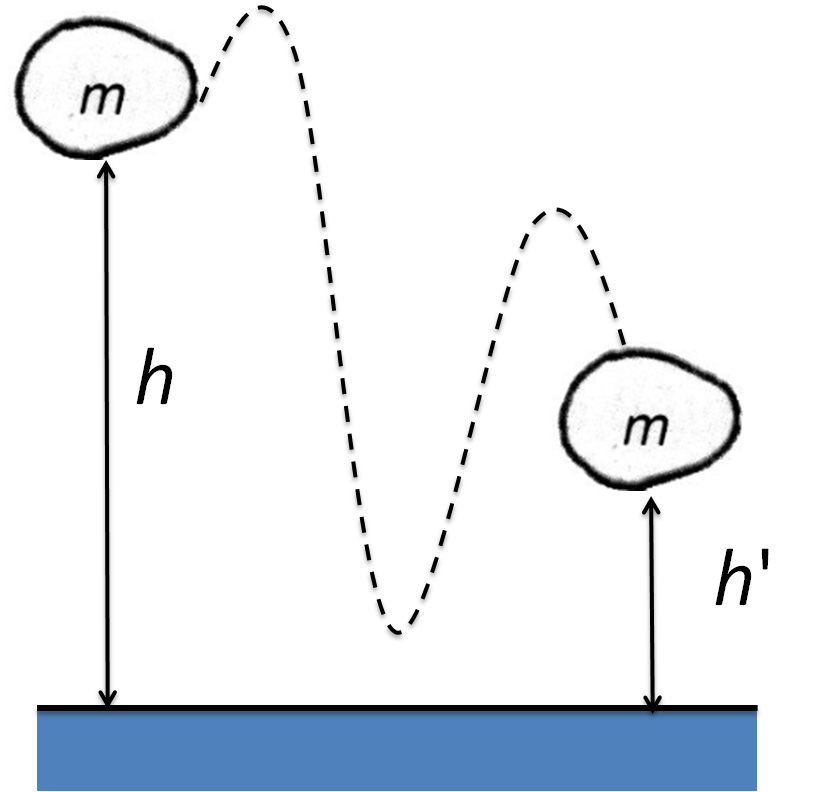
\includegraphics[scale=0.5]{img/potential-energy.eps}
  \caption{Gravity potential energy.}
  \label{fig:potential-energy}
\end{figure}

Figure \ref{fig:potential-energy} illustrated this concept.

We treat the Fibonacci heap pop operation in a similar
way, in order to evaluate the cost, we firstly define the potential
$\Phi(H)$ before extract the minimum element. This potential is
accumulated by insertion and merge operations executed so far.
And after tree consolidation and
we get the result $H'$, we then calculate the new potential $\Phi(H')$.
The difference between $\Phi(H')$ and $\Phi(H)$ plus the contribution
of consolidate algorithm indicates the amortized
performance of pop.

For pop operation analysis, the potential can be defined as

\be
\Phi(H) = t(H)
\ee

Where $t(H)$ is the number of trees in Fibonacci heap forest.
We have $t(H) = 1 + length(\mathbb{T})$ for any non-empty heap.

For the $n$-nodes Fibonacci heap, suppose there is an upper bound
of ranks for all trees as $D(n)$. After consolidation, it ensures
that the number of trees in the heap forest is at most $D(n)+1$.

Before consolidation, we actually did another important thing, which
also contribute to running time, we removed the root of the minimum
tree, and concatenate all children left to the forest. So consolidate
operation at most processes $D(n)+t(H)-1$ trees.

Summarize all the above factors, we deduce the amortized cost
as below.

\be
\begin{array}{lll}
T & = & T_{consolidation} + \Phi(H') -\Phi(H) \\
  & = & O(D(n)+t(H)-1) + (D(n) + 1) - t(H) \\
  & = & O(D(n))
\end{array}
\ee

If only insertion, merge, and pop function are applied to Fibonacci
heap. We ensure that all trees are binomial trees. It is easy to
estimate the upper limit $D(n)$ if $O(\lg n)$. (Suppose the extreme
case, that all nodes are in only one Binomial tree).

However, we'll show in next sub section that, there is operation can
violate the binomial tree assumption.

\subsection{Decreasing key}
\index{Fibonacci Heap!decrease key}
There is a special
heap operation left. It only makes sense for imperative settings.
It's about decreasing key of a certain node. Decreasing key plays
important role in some Graphic algorithms such as Minimum Spanning
tree algorithm and Dijkstra's algorithm \cite{CLRS}. In that case
we hope the decreasing key takes O(1) amortized time.

However, we can't define a function like $Decrease(H, k, k')$, which
first locates a node with key $k$, then decrease $k$ to $k'$ by replacement,
and then resume the heap properties. This is because the time for
locating phase is bound to $O(n)$ time, since we don't have a pointer
to the target node.

In imperative setting, we can define the algorithm as
\textproc{Decrease-Key}($H, x, k$). Here $x$ is a node in heap $H$, which
we want to decrease its key to $k$. We needn't perform a search, as
we have $x$ at hand. It's possible to give an amortized $O(1)$ solution.

When we decreased the key of a node, if it's not a root, this operation
may violate the property Binomial tree that the key of parent is
less than all keys of children. So we need to compare the decreased key
with the parent node, and if this case happens, we can cut this node
and append it to the root list. (Remind the recursive swapping solution
for binary heap which leads to $O(\lg n)$)

\begin{figure}[htbp]
  \centering
  \setlength{\unitlength}{1cm}
  \begin{picture}(12, 7)
    \put(0, 0){\includegraphics[scale=0.7]{img/cut-fib-tree.ps}}
    \put(6.7, 3){\line(1, 1){0.5}}
    \put(6.7, 3.5){\line(1, -1){0.5}}
  \end{picture}
  \caption{$x<y$, cut tree $x$ from its parent, and add $x$ to root list.} \label{fig:cut-fib-tree}
\end{figure}

Figure \ref{fig:cut-fib-tree} illustrates this situation. After decreasing
key of node $x$, it is less than $y$, we cut $x$ off its parent $y$, and
'past' the whole tree rooted at $x$ to root list.

Although we recover the property of that parent is less than all children,
the tree isn't any longer a Binomial tree after it losses some sub tree.
If a tree losses too many of its children because of cutting, we can't ensure
the performance of merge-able heap operations. Fibonacci Heap adds another
constraints to avoid such problem:

{\em If a node losses its second child, it is immediately cut from parent,
and added to root list}

The final \textproc{Decrease-Key} algorithm is given as below.

\begin{algorithmic}[1]
\Function{Decrease-Key}{$H, x, k$}
  \State \Call{Key}{$x$} $\gets k$
  \State $p \gets $ \Call{Parent}{$x$}
  \If{$p \neq NIL \land k < $ \Call{Key}{$p$}}
    \State \Call{Cut}{$H, x$}
    \State \Call{Cascading-Cut}{$H, p$}
  \EndIf
  \If{$k <$ \Call{Key}{$T_{min}(H)$}}
    \State $T_{min}(H) \gets x$
  \EndIf
\EndFunction
\end{algorithmic}

Where function \textproc{Cascading-Cut} uses the mark to determine
if the node is losing the second child. the node is marked after
it losses the first child. And the mark is cleared in \textproc{Cut}
function.

\begin{algorithmic}[1]
\Function{Cut}{$H, x$}
  \State $p \gets $ \Call{Parent}{$x$}
  \State remove $x$ from $p$
  \State \Call{Degree}{$p$} $\gets$ \Call{Degree}{$p$} - 1
  \State add $x$ to root list of $H$
  \State \Call{Parent}{$x$} $\gets NIL$
  \State \Call{Mark}{$x$} $\gets FALSE$
\EndFunction
\end{algorithmic}

During cascading cut process, if $x$ is marked, which means it has
already lost one child. We recursively performs cut and cascading cut
on its parent till reach to root.

\begin{algorithmic}[1]
\Function{Cascading-Cut}{$H, x$}
  \State $p \gets $ \Call{Parent}{$x$}
  \If{$p \neq NIL$}
    \If{\Call{Mark}{$x$} $= FALSE$}
      \State \Call{Mark}{$x$} $\gets TRUE$
    \Else
      \State \Call{Cut}{$H, x$}
      \State \Call{Cascading-Cut}{$H, p$}
    \EndIf
  \EndIf
\EndFunction
\end{algorithmic}

The relevant ANSI C decreasing key program is given as the following.

\lstset{language=C}
\begin{lstlisting}
void decrease_key(struct FibHeap* h, struct node* x, Key k){
  struct node* p = x->parent;
  x->key = k;
  if(p && k < p->key){
    cut(h, x);
    cascading_cut(h, p);
  }
  if(k < h->minTr->key)
    h->minTr = x;
}

void cut(struct FibHeap* h, struct node* x){
  struct node* p = x->parent;
  p->children = remove_node(p->children, x);
  p->degree--;
  h->roots = append(h->roots, x);
  x->parent = NULL;
  x->mark = 0;
}

void cascading_cut(struct FibHeap* h, struct node* x){
  struct node* p = x->parent;
  if(p){
    if(!x->mark)
      x->mark = 1;
    else{
      cut(h, x);
      cascading_cut(h, p);
    }
  }
}
\end{lstlisting}

\begin{Exercise}
Prove that \textproc{Decrease-Key} algorithm is amortized $O(1)$ time.
\end{Exercise}

\subsection{The name of Fibonacci Heap}
It's time to reveal the reason why the data structure is named
as 'Fibonacci Heap'.

There is only one undefined algorithm so far, \textproc{Max-Degree}($n$).
Which can determine the upper bound of degree for any node in a $n$ nodes
Fibonacci Heap. We'll give the proof by using Fibonacci series and
finally realize \textproc{Max-Degree} algorithm.

\begin{lemma}
\label{lemma:Fib-degree}
For any node $x$ in a Fibonacci Heap, denote $k = degree(x)$, and
$|x| = size(x)$, then
\be
  |x| \geq F_{k+2}
\ee

Where $F_k$ is Fibonacci series defined as the following.
\[
F_k = \left \{
  \begin{array}
  {r@{\quad:\quad}l}
  0 & k = 0 \\
  1 & k = 1 \\
  F_{k-1} + F_{k-2} & k \geq 2
  \end{array}
\right.
\]
\end{lemma}

\begin{proof}
Consider all $k$ children of node $x$, we denote them as $y_1, y_2, ..., y_k$
in the order of time when they were linked to $x$. Where $y_1$ is the
oldest, and $y_k$ is the youngest.

Obviously, $y_i \geq 0$. When we link $y_i$ to $x$, children $y_1, y_2, ..., y_{i-1}$ have already been there. And algorithm \textproc{LINK} only links
nodes with the same degree. Which indicates at that time, we have

\[
  degree(y_i) = degree(x) = i - 1
\]

After that, node $y_i$ can at most
lost 1 child, (due to the decreasing key operation) otherwise, if it
will be immediately cut off and append to root list after the second
child loss. Thus we conclude

\[
degree(y_i) \geq i-2
\]

For any $i = 2, 3, ..., k$.

Let $s_k$ be the {\em minimum possible size} of node $x$, where
$degree(x) = k$. For trivial cases, $s_0 = 1$, $s_1 = 2$, and we have

\bean
|x| & \geq & s_k \\
    & =   & 2 + \sum_{i=2}^{k} s_{degree(y_i)} \qquad \\
    & \geq & 2 + \sum_{i=2}^{k} s_{i-2}
\eean

We next show that $s_k > F_{k+2}$. This can be proved by induction.
For trivial cases, we have $s_0 = 1 \geq F_2 = 1$, and $s_1 = 2 \geq F_3 = 2$.
For induction case $k \geq 2$. We have

\bean
|x| & \geq & s_k \\
    & \geq & 2 + \sum_{i=2}^{k} s_{i-2} \\
    & \geq & 2 + \sum_{i=2}^{k} F_i \\
    & =    & 1 +  \sum_{i=0}^{k} F_i \\
\eean

At this point, we need prove that

\be
F_{k+2} = 1 +  \sum_{i=}^{k} F_i
\ee

This can also be proved by using induction:
\begin{itemize}
\item Trivial case, $F_2 = 1 + F_0 = 2$
\item Induction case,
\bean
  F_{k+2} & = & F_{k+1} + F_k \\
         & = & 1 + \sum_{i=0}^{k-1}F_i + F_k \\
         & = & 1 + \sum_{i=0}^{k} F_i
\eean
\end{itemize}

Summarize all above we have the final result.
\be
N \geq |x| \geq F_k+2
\ee
\end{proof}

Recall the result of AVL tree, that $F_k \geq \Phi^k$, where
$\Phi = \frac{1+\sqrt{5}}{2}$ is the golden ratio. We also proved
that pop operation is amortized $O(\lg n)$ algorithm.

Based on this result. We can define Function $MaxDegree$ as the following.

\be
  MaxDegree(n) = 1 + \lfloor \log_{\Phi} n \rfloor
\ee

The imperative \textproc{Max-Degree} algorithm can also be realized by
using Fibonacci sequences.

\begin{algorithmic}[1]
\Function{Max-Degree}{$n$}
  \State $F_0 \gets 0$
  \State $F_1 \gets 1$
  \State $k \gets 2$
  \Repeat
    \State $F_k \gets F_{k_1} + F_{k_2}$
    \State $k \gets k+1$
  \Until{$F_k < n$}
  \State \Return $k-2$
\EndFunction
\end{algorithmic}

Translate the algorithm to ANSI C given the following program.

\lstset{language=C}
\begin{lstlisting}
int max_degree(int n){
  int k, F;
  int F2 = 0;
  int F1 = 1;
  for(F=F1+F2, k=2; F<n; ++k){
    F2 = F1;
    F1 = F;
    F = F1 + F2;
  }
  return k-2;
}
\end{lstlisting}

% ================================================================
%                 Pairing Heaps
% ================================================================

\section{Pairing Heaps}
\label{pairing-heap} \index{Pairing heap}
Although Fibonacci Heaps provide excellent performance theoretically,
it is complex to realize. People find that the constant behind the
big-O is big. Actually, Fibonacci Heap is more significant in theory
than in practice.

In this section, we'll introduce another solution, Pairing heap,
which is one of the best heaps ever known in terms of performance.
Most operations including insertion, finding minimum element (top),
merging are all bounds to $O(1)$ time, while deleting minimum element (pop)
is conjectured to amortized $O(\lg n)$ time \cite{pairing-heap}
\cite{okasaki-book}. Note that this is still
a conjecture for 15 years by the time I write this chapter. Nobody has been
proven it although there are much experimental data support the
$O(\lg n)$ amortized result.

Besides that, pairing heap is simple. There exist both elegant
imperative and functional implementations.

% ================================================================
%                 Definition
% ================================================================
\subsection{Definition}
\index{Pairing heap!definition}

Both Binomial Heaps and Fibonacci Heaps are realized with forest.
While a pairing heaps is essentially a K-ary tree. The minimum element
is stored at root. All other elements are stored in sub trees.

The following Haskell program defines pairing heap.

\lstset{language=Haskell}
\begin{lstlisting}
data PHeap a = E | Node a [PHeap a]
\end{lstlisting}

This is a recursive definition, that a pairing heap is either empty
or a K-ary tree, which is consist of a root node, and a list of sub trees.

Pairing heap can also be defined in procedural languages, for example
ANSI C as below. For illustration purpose, all heaps we mentioned later
are minimum-heap, and we assume the type of key is integer \footnote{We
can parametrize the key type with C++ template, but this is beyond
our scope, please refer to the example programs along with
this book}. We use same linked-list based left-child, right-sibling
approach (aka, binary tree representation\cite{CLRS}).

\lstset{language=C}
\begin{lstlisting}
typedef int Key;

struct node{
  Key key;
  struct node *next, *children, *parent;
};
\end{lstlisting}

Note that the parent field does only make sense for decreasing key
operation, which will be explained later on. we can omit it for the
time being.


% ================================================================
%          Basic Heap operations
% ================================================================
\subsection{Basic heap operations}
In this section, we first give the merging operation for pairing
heap, which can be used to realize the insertion. Merging, insertion,
and finding the minimum element are relative trivial compare to
the extracting minimum element operation.

\subsubsection{Merge, insert, and find the minimum element (top)}
\index{Pairing heap!insert} \index{Pairing heap!top}
\index{Pairing heap!find min}
The idea of merging is similar to the linking algorithm we shown
previously for Binomial heap. When we merge two pairing heaps, there
are two cases.

\begin{itemize}
\item Trivial case, one heap is empty, we simply return the other
heap as the result;

\item Otherwise, we compare the root element of the two heaps, make
the heap with bigger root element as a new children of the other.
\end{itemize}

Let $H_1$, and $H_2$ denote the two heaps, $x$ and $y$ be the root
element of $H_1$ and $H_2$ respectively. Function $Children()$
returns the children of a K-ary tree. Function $Node()$ can
construct a K-ary tree from a root element and a list of children.

\be
merge(H_1, H_2) = \left \{
  \begin{array}
  {r@{\quad:\quad}l}
  H_1 & H_2 = \phi \\
  H_2 & H_1 = \phi \\
  Node(x, \{H_2\} \cup Children(H_1)) & x < y \\
  Node(y, \{H_1\} \cup Children(H_2)) & otherwise
  \end{array}
\right .
\ee

Where
\[
\begin{array}{l}
x = Root(H_1) \\
y = Root(H_2)
\end{array}
\]

It's obviously that merging algorithm is bound to $O(1)$ time
\footnote{Assume $\cup$ is constant time operation, this is true
for linked-list settings, including 'cons' like operation in
functional programming languages.}.
The $merge$ equation can be translated to the following Haskell program.

\lstset{language=Haskell}
\begin{lstlisting}
merge :: (Ord a) => PHeap a -> PHeap a -> PHeap a
merge h E = h
merge E h = h
merge h1@(Node x hs1) h2@(Node y hs2) =
    if x < y then Node x (h2:hs1) else Node y (h1:hs2)
\end{lstlisting}

Merge can also be realized imperatively. With left-child, right
sibling approach, we can just link the heap, which is in fact a
K-ary tree, with larger key as the first new child of the other.
This is constant time operation as described below.

\begin{algorithmic}[1]
\Function{Merge}{$H_1, H_2$}
  \If{$H_1 = $ NIL}
    \State \Return $H_2$
  \EndIf
  \If{$H_2 = $ NIL}
    \State \Return $H_1$
  \EndIf
  \If{\Call{Key}{$H_2$} $<$ \Call{Key}{$H_1$}}
    \State \Call{Exchange}{$H_1 \leftrightarrow H_2$}
  \EndIf
  \State Insert $H_2$ in front of \Call{Children}{$H_1$}
  \State \Call{Parent}{$H_2$} $\gets H_1$
  \State \Return $H_1$
\EndFunction
\end{algorithmic}

Note that we also update the parent field accordingly. The ANSI C
example program is given as the following.

\lstset{language=C}
\begin{lstlisting}
struct node* merge(struct node* h1, struct node* h2){
  if(h1 == NULL)
    return h2;
  if(h2 == NULL)
    return h1;
  if(h2->key < h1->key)
    swap(&h1, &h2);
  h2->next = h1->children;
  h1->children = h2;
  h2->parent = h1;
  h1->next = NULL; /*Break previous link if any*/
  return h1;
}
\end{lstlisting}

Where function swap() is defined in a similar way as Fibonacci Heap.

With merge defined, insertion can be realized as same as Fibonacci Heap
in Equation \ref{eq:fib-insert}. Definitely it's $O(1)$ time operation.
As the minimum element is always stored in root, finding it is trivial.

\be
top(H) = Root(H)
\ee

Same as the other two above operations, it's bound to $O(1)$ time.

\begin{Exercise}
Implement the insertion and top operation in your favorite programming
language.
\end{Exercise}

\subsubsection{Decrease key of a node}
\index{pairing heap!decrease key}
There is another trivial operation, to decrease key of a given node,
which only makes sense in imperative settings as we explained in Fibonacci
Heap section.

The solution is simple, that we can cut the node with the new smaller
key from it's parent along with all its children. Then merge it again
to the heap. The only special case is that if the given node is the
root, then we can directly set the new key without doing anything else.

The following algorithm describes this procedure for a given node $x$, with
new key $k$.

\begin{algorithmic}[1]
\Function{Decrease-Key}{$H, x, k$}
  \State \Call{Key}{$x$} $\gets k$
  \If{\Call{Parent}{$x$} $\neq$ NIL}
    \State Remove $x$ from \textproc{Children}(\Call{Parent}{$x$})
  \EndIf
  \Call{Parent}{$x$} $\gets$ NIL
  \State \Return \Call{Merge}{$H, x$}
\EndFunction
\end{algorithmic}

The following ANSI C program translates this algorithm.

\lstset{language=C}
\begin{lstlisting}
struct node* decrease_key(struct node* h, struct node* x, Key key){
  x->key = key; /* Assume key <= x->key */
  if(x->parent)
    x->parent->children = remove_node(x->parent->children, x);
  x->parent = NULL;
  return merge(h, x);
}
\end{lstlisting}

\begin{Exercise}
Implement the program of removing a node from the children of its
parent in your favorite imperative programming language. Consider
how can we ensure the overall performance of decreasing key is
O(1) time? Is left-child, right sibling approach enough?
\end{Exercise}

\subsubsection{Delete the minimum element from the heap (pop)}
\index{Pairing heap!pop} \index{Pairing heap!delete min}
Since the minimum element is always stored at root, after delete it
during popping, the rest things left are all sub-trees. These trees
can be merged to one big tree.

\be
  pop(H) = mergePairs(Children(H))
\ee

Pairing Heap uses a special approach that it merges every two sub-trees
from left to right in pair. Then
merge these paired results from right to left which forms a final
result tree. The name of `Pairing Heap' comes from the characteristic
of this pair-merging.

Figure \ref{fig:merge-pairs} and \ref{fig:merge-right} illustrate the procedure of pair-merging.

\begin{figure}[htbp]
  \centering
  \subfloat[A pairing heap before pop.]{\includegraphics[scale=0.5]{img/pairing-hp.ps}} \\
  \subfloat[After root element 2 being removed, there are 9 sub-trees left.]{\includegraphics[scale=0.5]{img/pairs.ps}} \\
  \subfloat[Merge every two trees in pair, note that there are odd number trees, so the last one needn't merge.]{\includegraphics[scale=0.5]{img/pairs-merge.ps}} \\
  \caption{Remove the root element, and merge children in pairs.} \label{fig:merge-pairs}
\end{figure}

\begin{figure}[htbp]
  \centering
  \subfloat[Merge tree with 9, and tree with root 6.]{\hspace{0.2\textwidth}\includegraphics[scale=0.5]{img/right-merge-1.ps}\hspace{0.2\textwidth}}
  \subfloat[Merge tree with root 7 to the result.]{\hspace{0.1\textwidth}\includegraphics[scale=0.5]{img/right-merge-2.ps}\hspace{0.1\textwidth}} \\
  \subfloat[Merge tree with root 3 to the result.]{\hspace{0.1\textwidth}\includegraphics[scale=0.5]{img/right-merge-3.ps}\hspace{0.1\textwidth}}
  \subfloat[Merge tree with root 4 to the result.]{\hspace{0.1\textwidth}\includegraphics[scale=0.5]{img/right-merge-4.ps}\hspace{0.1\textwidth}}
  \caption{Steps of merge from right to left.} \label{fig:merge-right}
\end{figure}

The recursive pair-merging solution is quite similar to the bottom up
merge sort\cite{okasaki-book}. Denote the children of a pairing
heap as $A$, which is a list of trees of $\{ T_1, T_2, T_3, ..., T_m\}$
for example. The $mergePairs()$ function can be given as below.

\be
mergePairs(A) = \left \{
  \begin{array}
  {r@{\quad:\quad}l}
  \Phi & A = \Phi \\
  T_1 & A = \{ T_1 \} \\
  merge(merge(T_1, T_2), mergePairs(A')) & otherwise
  \end{array}
\right .
\ee

where

\[
A' = \{ T_3, T_4, ..., T_m\}
\]

is the rest of the children without the first two trees.

The relative Haskell program of popping is given as the following.

\lstset{language=Haskell}
\begin{lstlisting}
deleteMin :: (Ord a) => PHeap a -> PHeap a
deleteMin (Node _ hs) = mergePairs hs where
    mergePairs [] = E
    mergePairs [h] = h
    mergePairs (h1:h2:hs) = merge (merge h1 h2) (mergePairs hs)
\end{lstlisting}

The popping operation can also be explained in the following
procedural algorithm.

\begin{algorithmic}[1]
\Function{Pop}{$H$}
  \State $L \gets NIL$
  \For{every 2 trees $T_x$, $T_y \in$ \Call{Children}{$H$} from left to right}
    \State Extract $x$, and $y$ from \Call{Children}{$H$}
    \State $T \gets $ \Call{Merge}{$T_x, T_y$}
    \State Insert $T$ at the beginning of $L$
  \EndFor
  \State $H \gets $ \Call{Children}{$H$} \Comment{$H$ is either $NIL$ or one tree.}
  \For{$\forall T \in L$ from left to right}
    \State $H \gets $ \Call{Merge}{$H, T$}
  \EndFor
  \State \Return $H$
\EndFunction
\end{algorithmic}

Note that $L$ is initialized as an empty linked-list, then the algorithm
iterates every two trees in pair in the children of the K-ary tree, from
left to right, and performs merging, the result is inserted at the beginning
of $L$. Because we insert to front end, so when we traverse $L$ later on,
we actually process from right to left. There may be odd number of sub-trees
in $H$, in that case, it will leave one tree after pair-merging. We
handle it by start the right to left merging from this left tree.

Below is the ANSI C program to this algorithm.

\lstset{language=C}
\begin{lstlisting}
struct node* pop(struct node* h){
  struct node *x, *y, *lst = NULL;
  while((x = h->children) != NULL){
    if((h->children = y = x->next) != NULL)
      h->children = h->children->next;
    lst = push_front(lst, merge(x, y));
  }
  x = NULL;
  while((y = lst) != NULL){
    lst = lst->next;
    x = merge(x, y);
  }
  free(h);
  return x;
}
\end{lstlisting}

The pairing heap pop operation is conjectured to be amortized $O(\lg n)$
time \cite{pairing-heap}.

\begin{Exercise}
Write a program to insert a tree at the beginning of a linked-list
in your favorite imperative programming language.
\end{Exercise}

\subsubsection{Delete a node}
\index{pairing heap!delete}
We didn't mention delete in Binomial heap or Fibonacci Heap. Deletion
can be realized by first decreasing key to minus infinity ($-\infty$), then
performing pop. In this section, we present another solution for
delete node.

The algorithm is to define the function $delete(H, x)$, where $x$ is
a node in a pairing heap $H$ \footnote{Here the semantic of $x$ is a
reference to a node.}.

If $x$ is root, we can just perform a pop operation. Otherwise, we
can cut $x$ from $H$, perform a pop on $x$, and then merge the pop
result back to $H$. This can be described as the following.

\be
delete(H, x) = \left \{
  \begin{array}
  {r@{\quad:\quad}l}
  pop(H) & x \quad \text{is root of} \quad H \\
  merge(cut(H, x), pop(x)) & otherwise
  \end{array}
\right .
\ee

As delete algorithm uses pop, the performance is conjectured to be
amortized $O(1)$ time.

\begin{Exercise}
\begin{itemize}
\item Write procedural pseudo code for delete algorithm.

\item Write the delete operation in your favorite imperative programming
language

\item Consider how to realize delete in purely functional setting.
\end{itemize}
\end{Exercise}

% ================================================================
%                 Short summary
% ================================================================
\section{Notes and short summary}

In this chapter, we extend the heap implementation from binary tree to
more generic approach. Binomial heap and Fibonacci heap use Forest of
K-ary trees as under ground data structure, while Pairing heap use
a K-ary tree to represent heap. It's a good point to post pone some
expensive operation, so that the over all amortized performance is
ensured. Although Fibonacci Heap gives good performance in theory, the
implementation is a bit complex. It was removed in some latest textbooks.
We also present pairing heap, which is easy to realize and have good
performance in practice.

The elementary tree based data structures are all introduced in this
book. There are still many tree based data structures which we can't
covers them all and skip here. We encourage the reader to refer to
other textbooks about them. From next chapter, we'll introduce generic
sequence data structures, array and queue.

% ================================================================
%                 Appendix
% ================================================================

\begin{thebibliography}{99}

\bibitem{K-ary-tree}
K-ary tree, Wikipedia. http://en.wikipedia.org/wiki/K-ary\_tree

\bibitem{CLRS}
Thomas H. Cormen, Charles E. Leiserson, Ronald L. Rivest and Clifford Stein. ``Introduction to Algorithms, Second Edition''. The MIT Press, 2001. ISBN: 0262032937.

\bibitem{okasaki-book}
Chris Okasaki. ``Purely Functional Data Structures''. Cambridge university press, (July 1, 1999), ISBN-13: 978-0521663502

\bibitem{wiki-pascal-triangle}
Wikipedia, ``Pascal's triangle''. http://en.wikipedia.org/wiki/Pascal's\_triangle

\bibitem{hackage-fibq}
Hackage. ``An alternate implementation of a priority queue based on a Fibonacci heap.'', http://hackage.haskell.org/packages/archive/pqueue-mtl/1.0.7/doc/html/src/Data-Queue-FibQueue.html

\bibitem{okasaki-fibh}
Chris Okasaki. ``Fibonacci Heaps.'' http://darcs.haskell.org/nofib/gc/fibheaps/orig

\bibitem{pairing-heap}
Michael L. Fredman, Robert Sedgewick, Daniel D. Sleator, and Robert E. Tarjan. ``The Pairing Heap: A New Form of Self-Adjusting Heap'' Algorithmica (1986) 1: 111-129.

\end{thebibliography}

\ifx\wholebook\relax \else
\end{document}
\fi
